%! TEX program = pdflatex

\documentclass[oneside,solution]{karazin-complan-assign}

\usepackage[utf8]{inputenc}
\usepackage[english,ukrainian]{babel}

\title{Контрольна робота}
\author{Захаров Дмитро}
\studentID{МП-31}
\instructor{Гиря Н.П.}
\date{\today}
\duedate{10:00 27 травня, 2024}
\assignno{2}
\semester{Весняний семестр 2024}
\mainproblem{Перетворення. Варіант 4}

\begin{document}

\maketitle

% \startsolution[print]

\problem{Лінійно-дробова функція \#1}

\hspace{20px}\textbf{Умова.} Знайти лінійно-дробове відображення $\omega: \hat{\mathbb{C}} \to \hat{\mathbb{C}}$ таке, що задовільняє $\omega(0)=1+i, \omega(2)=\infty, \omega(1+i)=3$.

\textbf{Розв'язання.} Як відомо, існує єдине лінійне-дробове відображення таке, що переводить трійку заданих точок в іншу трійок точок. Для знаходження $\omega$ скористаємось співвідношенням
\begin{equation}
    \omega: \frac{z-z_1}{z-z_2} \cdot \frac{z_3-z_2}{z_3-z_1} = \frac{\omega - \omega_1}{\omega - \omega_2} \cdot \frac{\omega_3-\omega_2}{\omega_3-\omega_1}
\end{equation}

Власне, залишається лише підставити наші точки:
\begin{equation}
    \frac{z-0}{z-2} \cdot \frac{1+i-2}{1+i-0} = \frac{\omega - (1+i)}{\omega - \infty} \cdot \frac{3-\infty}{3-(1+i)}
\end{equation}

Тут виникає питання з тим, що робити з виразами типу $\omega-\infty$. Правило наступне: вирази, де є точка на нескінченності, треба заміняти одиничкою. Тому остаточно маємо:
\begin{equation}
    \frac{z}{z-2} \cdot \frac{-1+i}{1+i} = \frac{\omega - (1+i)}{2-i}
\end{equation}

Оскільки $\frac{-1+i}{1+i} = i$, то можна спростити до:
\begin{gather}
    \omega = (2-i) \cdot \frac{iz}{z-2} + (1 + i) = \frac{(2i+1)z + (1+i)(z-2)}{z-2} \\
    = \boxed{\frac{(2+3i)z-2(1+i)}{z-2}}
\end{gather}

\textbf{Відповідь.} $\omega=\frac{(2+3i)z-2(1+i)}{z-2}$

\problem{Перетворення}

\hspace{20px}\textbf{Умова.} Перевести область $\mathcal{D} = \{z \in \mathbb{C}: |\text{Im}(z)| < \pi \wedge z \neq (\pi,+\infty) \cup (-\infty,0)\}$ на верхню напівплощину.

\textbf{Відповідь.} Спочатку застосуємо експоненійне відображення $z \mapsto e^z$. Тоді прямі $z=x\pm i\pi$ перейдуть у $e^{x \pm i\pi} = e^{\pm i\pi}e^x=-e^x, x \in \mathbb{R}$. Це відповідає променю $(-\infty,0)$. Тобто, $z \neq (-\infty,0)$. Відрізок $(-\infty, 0)$ перейде у $(0,1)$, а $(\pi,+\infty)$ у $(e^{\pi},+\infty)$. Отже, маємо Рисунок \ref{fig:2(1)}.

\begin{figure}
    \centering
    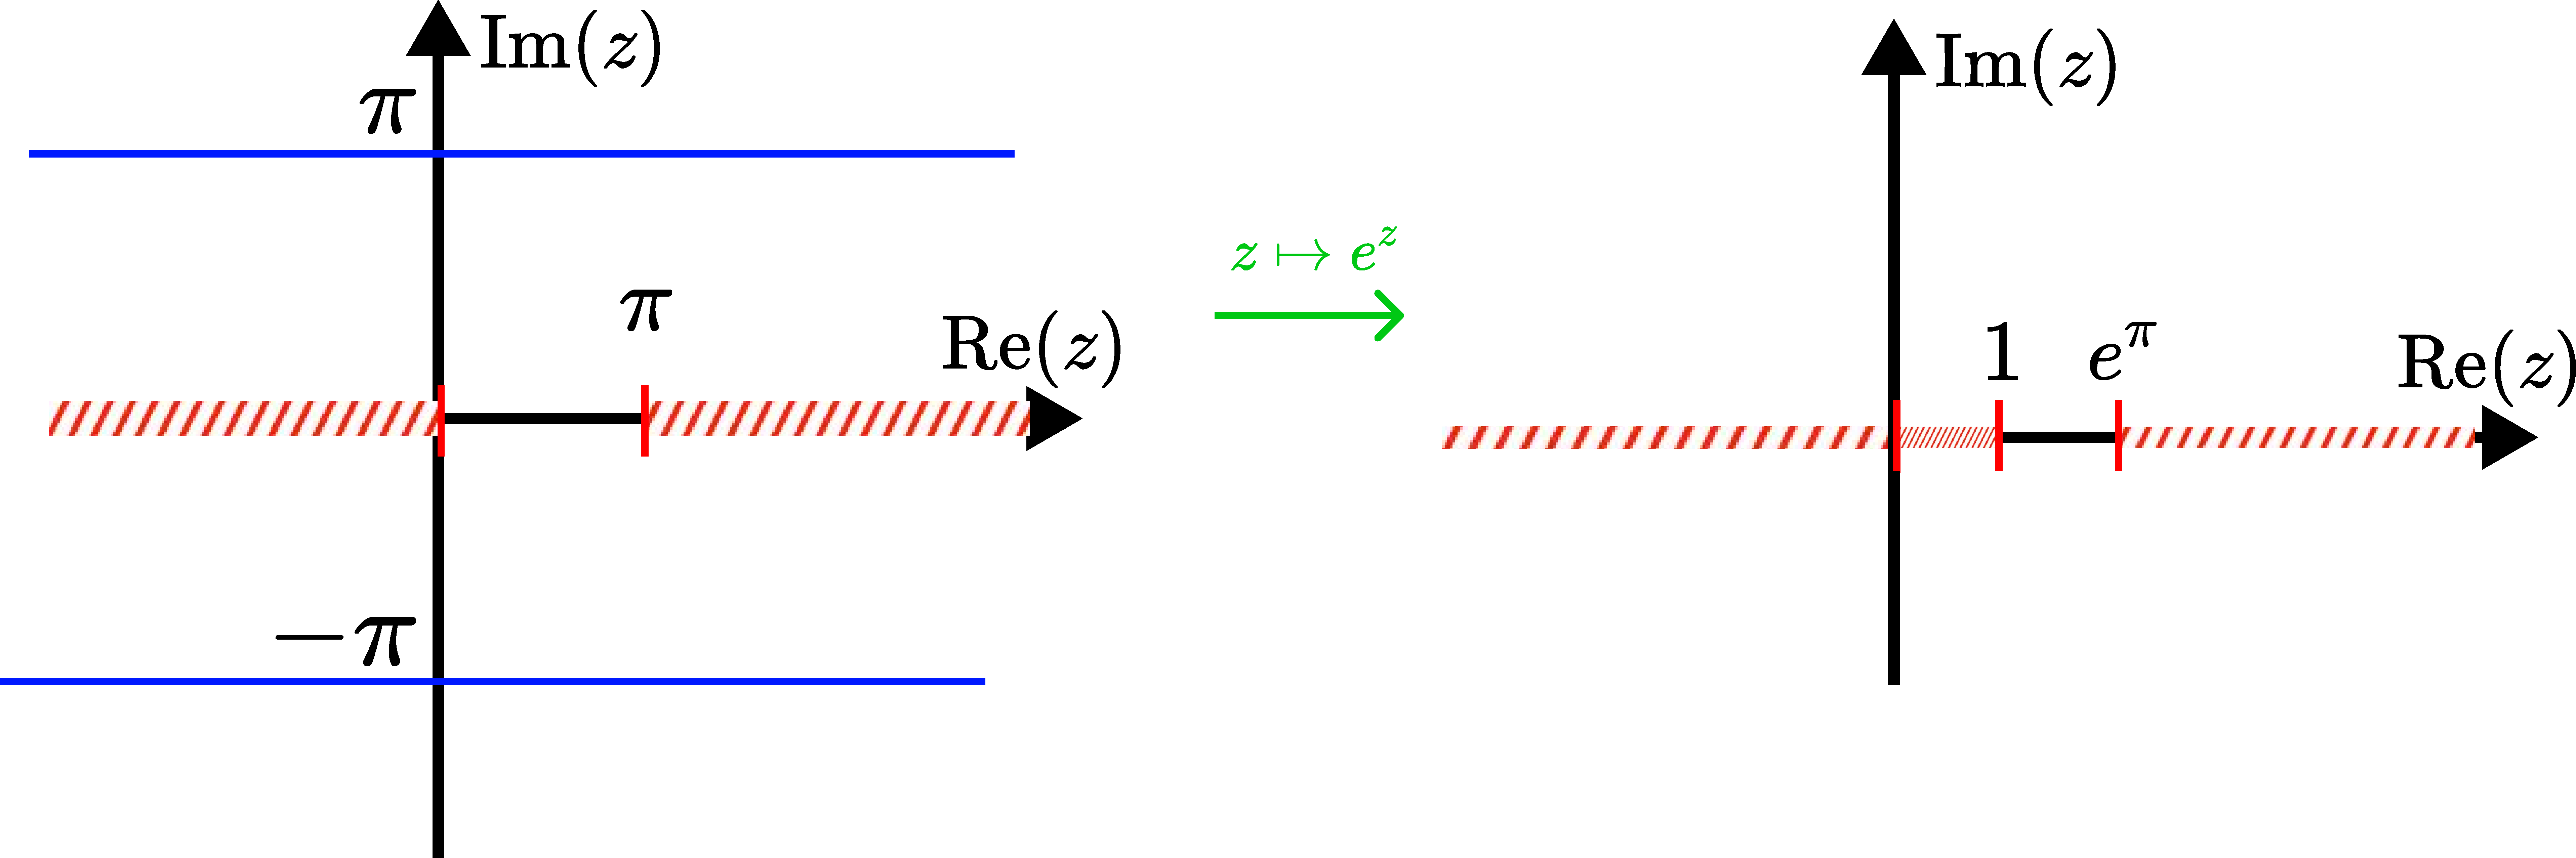
\includegraphics[width=\textwidth]{images/test_2/plot_2_1.pdf}
    \caption{Перетворення $z \mapsto e^z$ до початкового образу в задачі 2.}
    \label{fig:2(1)}
\end{figure}

Отже, по суті треба перевести $z \neq (-\infty, 1) \cup (e^{\pi},+\infty)$ до $z \neq (-\infty,-1) \cup (1,+\infty)$, а далі застосувати обернену функцію Жуковсього. Для цього віднімемо $\frac{1+e^{\pi}}{2}$, це переведе нашу область в $z \neq (-\infty, \frac{1}{2}-\frac{e^{\pi}}{2}) \cup (\frac{e^{\pi}}{2} - \frac{1}{2})$. Ділимо на $\frac{e^{\pi}-1}{2}$, отримаємо $z \neq (-\infty, 1) \cup (1,+\infty)$, а далі засувавши функцію Жуковсього, отримаємо результат. Отже, перші два перетворення мають вигляд:
\begin{equation}
    z \mapsto \frac{e^{\pi}-1}{2}\left(z-\frac{1+e^{\pi}}{2}\right)
\end{equation}

А далі $z \mapsto z+\sqrt{z^2-1}$. Весь процес проілюстровано на Рисунку \ref{fig:2(2)}. Наше відображення тоді доволі об'ємне, тому явно його не будемо виписувати.

Дещо більш просте перетворення можна отримати за допомогою дробово-лінійного відображення. Якщо спочатку застосувати $z \mapsto \frac{z-e^{\pi}}{z-1}$ ($1 \mapsto \infty, e^{\pi} \mapsto 0$), а далі взяти корінь з цього, то теж отримаємо шуканий результат. Тобто, $\omega(z) = \sqrt{\frac{e^z - e^{\pi}}{e^{z}-1}}$.

\begin{figure}
    \centering
    
\includegraphics[width=\textwidth]{images/test_2/plot_2_2.pdf}
    \caption{Перетворення, що закінчує задачу 2.}
    \label{fig:2(2)}
\end{figure}

\problem{Гіперболічний косинус}

\hspace{20px}\textbf{Умова.} Знайти образ при застосуванні відображення $\omega: z \mapsto \cosh z$ на область $\mathcal{D} = \{z \in \mathbb{C}: \text{Re}(z) > 0 \wedge -1 < \text{Im}(z) < 0\}$.

\textbf{Коментар.} У завданні було написано $\cosh \pi$ замість відображення, тому я підозрюю, що там мало стояти $\cosh z$.

\textbf{Розв'язання.} Як відомо, гіперболічний косинус можна записати за означенням як $\omega(z)=\frac{e^z + e^{-z}}{2}$. Тепер помітимо, що по суті, ми маємо композицію двох перетворень:
\begin{itemize}
    \item Спочатку накладається експоненційне відображення $z \mapsto e^z$.
    \item Далі накладається функція Жуковського $z \mapsto \frac{1}{2}\left(z+\frac{1}{z}\right)$.
\end{itemize}

Отже, залишається послідовно накласти ці два відображення до заданої області $\mathcal{D}$.

\textbf{Крок 1.} Розглянемо, як перетворюються границі області при такому перетворенні. Дійна пряма $(0,+\infty)$ перейде у відрізок $(1,+\infty)$. Горизональна пряма $x-i$ для $x \in (0,+\infty)$ перетвориться на $e^{x-i}=e^xe^{-i} = z_0e^x$ -- це буде промінь від початку координат до $z_0$, починаючи з $z_0$, де $z_0=e^{-i}$. 

\begin{figure}
    \centering
    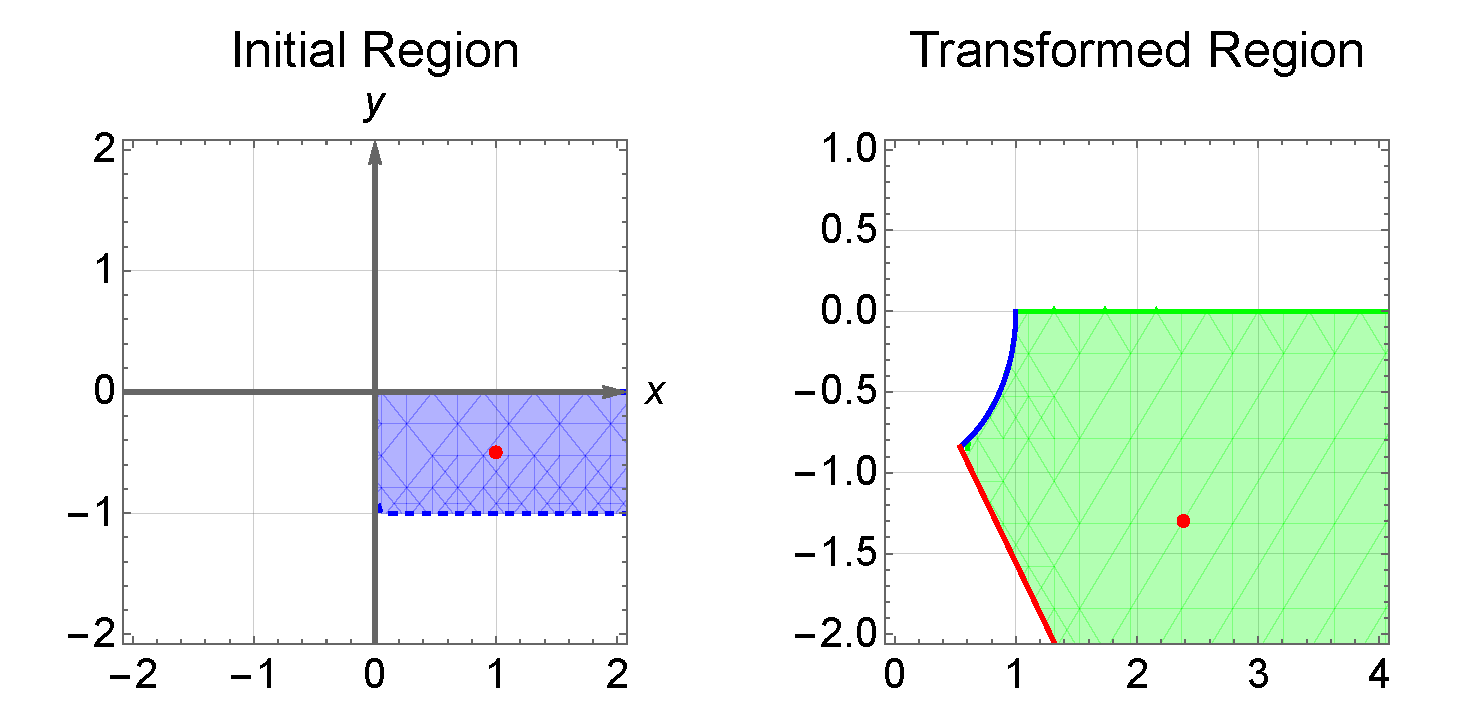
\includegraphics[width=\textwidth]{images/test_2/plot_3_1.pdf}
    \caption{Перетворення $z \mapsto e^z$ до початкового образу в задачі 3.}
    \label{fig:3(1)}
\end{figure}

Вертикальна пряма $it$ для $t \in (-1,0)$, тому образом буде дуга на одиничному колі між $1$ та $e^{-i}$. 

Нарешті, щоб визначити орієнтацію, підставимо якусь точку. Наприклад, $i\pi \notin \mathcal{D}$. Тоді $e^{i\pi}=-1$ не належить області, а отже маємо Рисунок \ref{fig:3(1)}. 

\textbf{Крок 2.} Застосовуємо функцію Жуковсього на дугу та дві прямі. Дугу одиничного колу функція Жуковсього переводить на відрізок. Один кінець це $z=1$, а інший $\frac{1}{2}(e^i+e^{-i})=\cos 1$, тобто маємо відрізок $(\cos 1, 1)$. Далі промінь $z=t$ для $t \in (1,+\infty)$ відобразиться на промінь $(1,+\infty)$. 

Нарешті, $z=z_0t$ для $t \in (1,+\infty)$ перейде у:
\begin{equation}
    \phi: z_0t \mapsto \frac{1}{2}\left(z_0t + \frac{1}{z_0t}\right) = \frac{1}{2}\left(e^{-i}t + \frac{e^i}{t}\right)
\end{equation}

Отже, можемо знайти конкретний параметричний вигляд образу. Наприклад, дійсна частина:
\begin{equation}
    \text{Re}(\phi(t)) = t \cos 1 + \frac{\cos 1}{t}, \; \text{Im}(\phi(t)) = -t \sin 1 + \frac{\sin 1}{t}
\end{equation}

Скоріше за все, цю криву можна віднести до якогось конкретного класу (наприклад, гіперболи), але явно я це не побачив, тому її і побудував. Результат на Рисунку \ref{fig:3(2)}. Область має бути замальованою всередині, під прямою $y=0$.

\begin{figure}
    \centering
    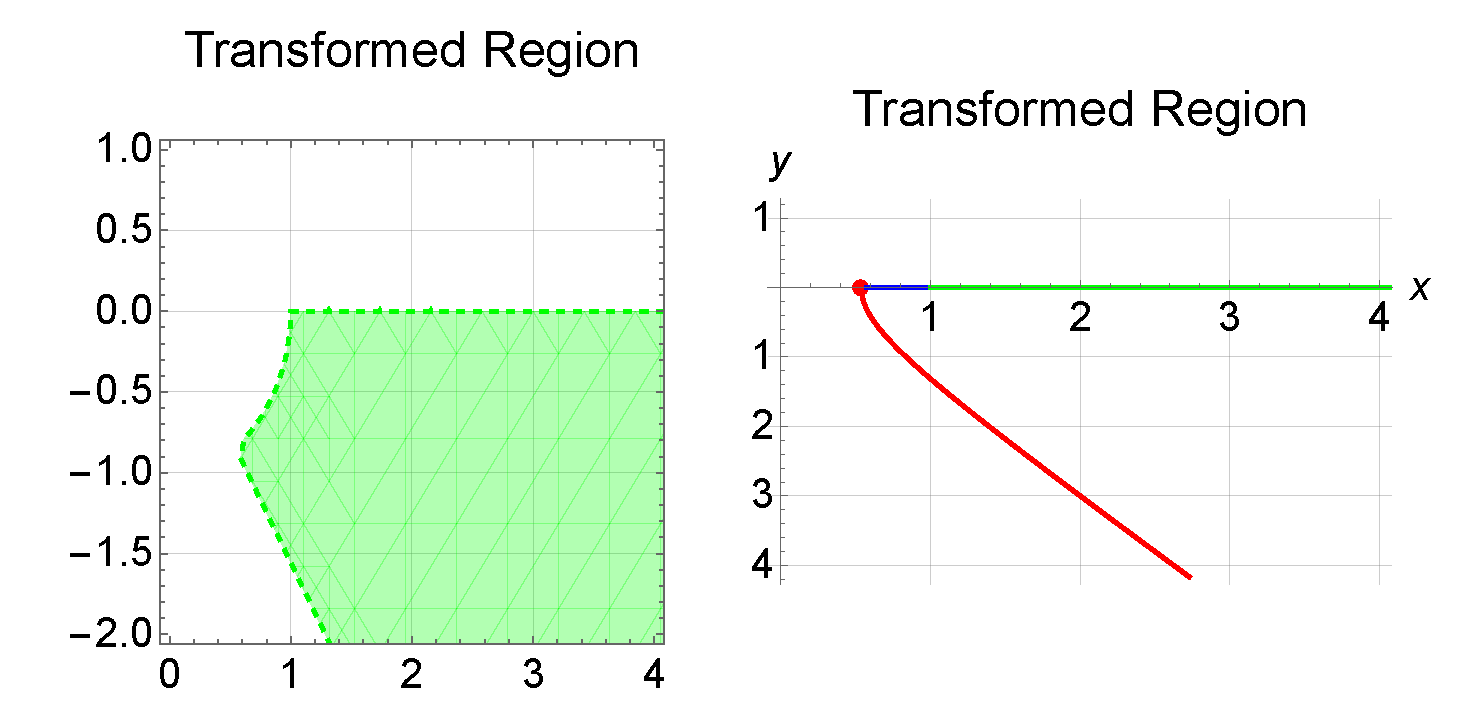
\includegraphics[width=\textwidth]{images/test_2/plot_3_2.pdf}
    \caption{Перетворення Жуковського до першого образу в задачі 3.}
    \label{fig:3(2)}
\end{figure}

\problem{Лінійно-дробова функція \#2}

\hspace{20px}\textbf{Умова.} Знайти образ при застосуванні відображення $\omega: z \mapsto \frac{2+z}{z+1}$ на область $\mathcal{D} = \{z \in \mathbb{C}: |z+1|>2\}$.

\textbf{Розв'язання.} Як відомо, лінійно-дробове відображення переводить узагальнене коло у узагальнене коло. Це означає, що як результат ми або отримаємо інше коло, або пряму. 

Помітимо, що у нашого лінійно-дробового відображення $\omega: z \mapsto \frac{2+z}{z+1}$ є особлива точка $z=-1$. Причому, $-1$ не належить нашій області і границі (а точніше, вона є центром кола $|z+1|=2$).

За принципом симетрії, знайдемо центр відображення $\omega(\mathcal{D})$. Симетричним до центра кола є точка на нескінченності і навпаки. Тому, $\omega(\infty)$ має відповідати центру нового відображення. Легко бачити, що $\omega(\infty)=1$ -- отже це новий центр.

Отже, залишилося знайти радіус. Як відомов, дві точки $z$ та $z^*$ є симетричними відносно кола, якщо $|z-z_0|\cdot|z^*-z_0|=R^2$. Тому візьмемо дві симетричні точки, вони переведуться у інші дві симетричні точки, а звідти ми знайдемо радіус.

Отже, нехай $z=0$, тоді $1 \cdot |z^*+1|=4$ звідси $z^*=3$ ($z^*=-5$ буде лежати на іншому промені). Тоді нова пара симетричних точок $\omega(0)=2, \omega(3)=\frac{5}{4}$. Тому, радіус знайдемо як:
\begin{equation}
    \left(2-1\right)\left(\frac{5}{4}-1\right) = (R^*)^2 \implies R^* = \frac{1}{2}
\end{equation}

Отже, залишається лише знайти орієнтацію. Підставимо, наприклад, $2 \in \mathcal{D}$. Тоді $\omega(2) = \frac{4}{3}$ -- належить всередині знайденого кола.

Отже остаточно наш образ $|z-1|<\frac{1}{2}$.

\begin{figure}
    \centering
    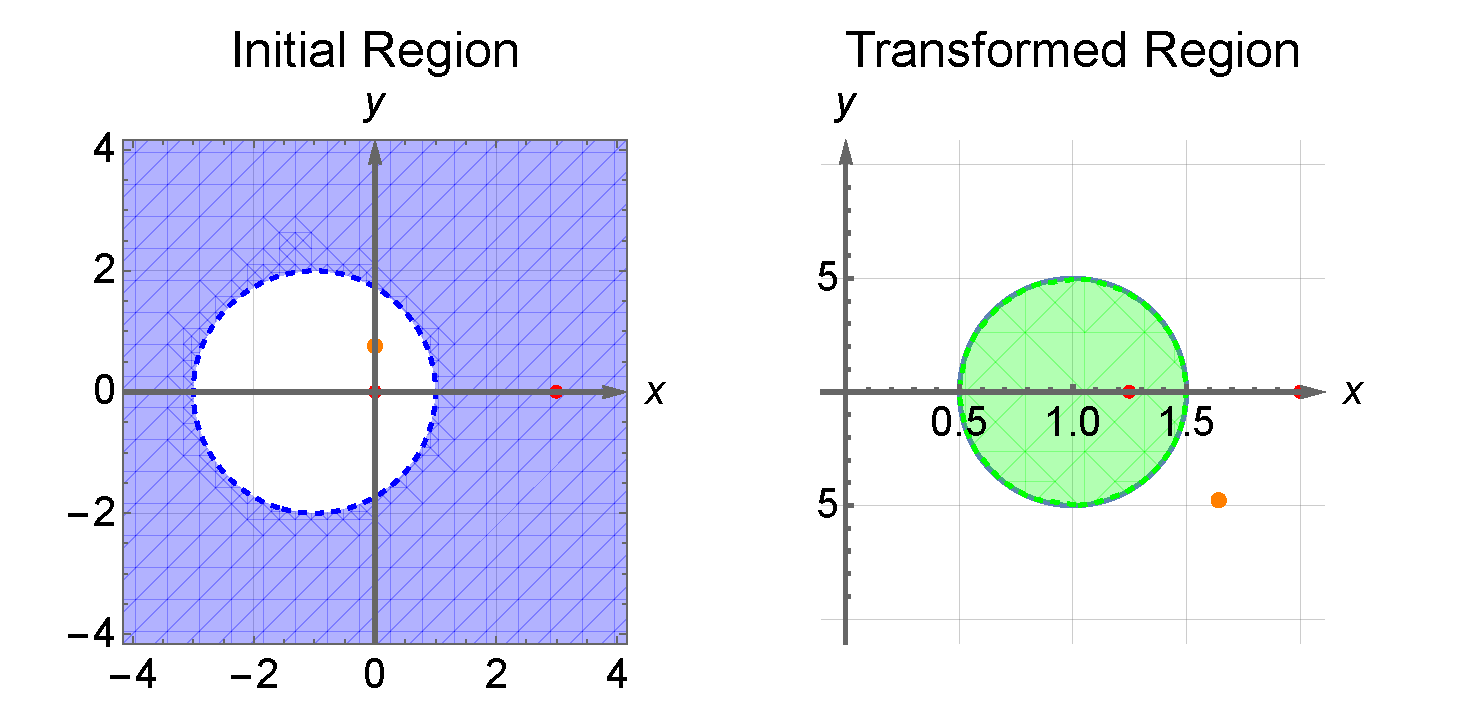
\includegraphics[width=\textwidth]{images/test_2/plot_4.pdf}
    \caption{Перетворення в задачі 4. Червоним відмічено симетричні точки до і після перетворення, помаранчевим -- якась точка за областю.}
    \label{fig:2(1)}
\end{figure}

\textbf{Відповідь.} $\{z \in \mathbb{C}: |z-1|<\frac{1}{2}\}$.

\end{document}
